\documentclass{article}

\usepackage[utf8]{inputenc}
\usepackage{placeins}
\usepackage{graphicx}
\usepackage[ruled,vlined,linesnumbered]{algorithm2e}
\usepackage{listings}
\usepackage{amsthm}
\usepackage{amsmath}
\usepackage{caption}
\usepackage{epigraph}

\captionsetup[figure]{font=scriptsize}

\newtheorem{definition}{Definição}[section]
\theoremstyle{remark}
\newtheorem*{remark}{Observações}
\theoremstyle{theorem}
\newtheorem{theorem}{Teorema}[section]

\setlength{\parskip}{.5em}

\renewcommand\refname{Leituras adicionais}
\renewcommand\figurename{Figura}
\renewcommand{\lstlistingname}{Código}

\newcommand{\eclipse}{$ECL^iPS^e$}
\newcommand{\definicao}[1]{\textbf{#1}\marginpar{\small \textbf{#1}}}

\lstdefinestyle{prosty}{
  language=Prolog,
  basicstyle=\small
}



\begin{document}

\section{Heurísticas}

Nos métodos de busca vistos até agora, a ordem de variáveis adotada é a ordem apresentada na lista
e a ordem de valores para cada variável é fixa. Para problemas maiores, pode ser mais conveniente
considerar ordenações diferentes para cada tipo de problema. Essas ordenações são geralmente
escolhidas de forma heurística e, por isso, são chamadas ordenações heurísticas. Existem,
naturalmente, duas classes de ordenações heurísticas: ordenação heurística de variáveis e de
valores.

Mas, antes de prosseguirmos, será útil falarmos sobre vetores, que serão utilizados nos programas a
seguir.

\subsection{Vetores}

Listas são interessantes, mas, eventualmente, podemos querer realizar acesso em tempo constante aos
seus membros, o que não é possível. Em outras linguagens, esse tipo de acesso é por costume
realizado através de vetores. Vetores existem em Prolog padrão, de certa forma. Como os argumentos
de funtores podem ser acessados em tempo constante por meio do funtor \funtor{arg/3}, a princípio,
um funtor qualquer poderia ser usado como um vetor, o acesso aos membros do qual feitos por meio de
\funtor{arg/3}. Essa abordagem, no entanto, não só não parece muito elegante, como é pouco prática.
Se temos algo que chamamos de vetor, gostaríamos de poder fazer algo como \codigo{ Vetor =/= 4}, por
exemplo, o que com os meios do Prolog padrão não é possível.

Para esse tipo de situação, no \eclipse existe uma implementação de vetores como um açucar
sintático (semelhante ao que vimos na implementação de listas), permitindo justamente esse tipo de
utilizaçãoa. Em particular, um vetor, é escrito como uma variável seguida do funtor de lista (como
em \codigo{Var[4]}), ou, se anônimo, como \codigo{[](A, B, C)} (note que, assim, a representação de
um vetor ou de uma lista vazia é a mesma) Para criar ``vetores'', possivelmente multidimensionais
(na realidade, matrizes, o que justifica os ``''), foi construído o predicado \funtor{dim/2}, que
pode ser usado ou para criar vetores ou para extrair sua dimensão.

\subsection{As n-rainhas}

Analisaremos o efeito de algumas heurísticas pela resolução do \enphasis{problema das
  n-rainhas} quando $n \geq 3$\footnote{Quando n = 2 ou n = 3, o problema não tem solução}. É um
problema por restrições tão bem conhecido que um estudante de programação por
restrições poderia (e com razão) se sentir enganado se terminasse um livro sobre o tema sem saber
como resolver esse problema em especial. A discussão a seguir é baseada, em grande parte, em
\cite{krzysztof}.

Para quem não conhece, o \enphasis{problema das n-rainhas} é o problema de alocar n rainhas em um
tabuleiro como o de xadrez, mas $n\times n$, com a restrição de que as rainhas não tem permissão
para se atacarem segundo as regras usuais de xadrez.

Existe um algoritmo polinomial para a resolução desse problema (que não veremos aqui), mas o que
veremos muitas vezes é mais conveniente e até mais rápido. Antes de considerarmos o papel das
heurística, vejamos como é uma solução mais simples. Notamos primeiro que, como temos n rainhas,
precisa existir uma rainha em cada linha e em cada coluna. Ou seja, para cada coluna (ou cada linha)
só precisamos indicar em qual linha (coluna) a rainha está, o que significa que a solução requer um
lista\footnote{Ou um vetor.} de n posições, não uma matriz (como alguém podria supor a princípio). O domínio de cada
posição na lista é o intervalo inteiro $[1,n]$ e as restrições são que só pode existir uma rainha
por linha (ou por coluna), o que se traduz na restrição \codigo{alldifferent(Cols)}, em que
\var{Cols} é o vetor de colunas. Ademais, só pode existir uma rainha por linha, o que se traduz nas
restrições \codigo{$X_i$ - $X_j$ $\setminus=\setminus$ I - J} e \codigo{$X_i$ - $X_j$
  $\setminus=\setminus$ J - I}, em que $X_i$ e $X_j$ são membros distintos da lista de colunas (ou linhas).

    \begin{listing}[!h]
    \inputminted{prolog}{../Exemplos/Cap11/prog1_queens.ecl}
    \caption{Queens}
    \end{listing}

Esse programa primeiro declara o vetor \var{RainhaStruct}, impõe a ele as restrições mencionadas,
transforma o vetor em lista e realiza a busca (como explicada no Capítulo 10).%TODO por link
O programa, no computador do autor, consegue resolver o problema por esse programa para N até 29,
mas, adotando um tempo limite de 50 segundos, N = 30 já está fora de mão.

Alguém poderia dizer que isso ocorre porque esse código não foi feito de maneira inteligente,
já que a assimetria do problema, presente no fato de que a alocação de uma rainha em uma coluna
central, por exemplo, resulta em maiores restrições nas posições das outras rainhas, não está
representada no código. Esse realmente é o caso e, para fazê-lo deixar de ser, criamos uma nova
versão do programa.

\subsection{Ordenação de variáveis}

A alteração consiste na adição de um argumento Heur (de heurística) no predicado \funtor{rainhas/2} (que se torna
\funtor{rainhas/3}). Esse predicado nos diz qual a heurística usada para ordenar as variáveis.
Podemos definir o \funtor{rainhas/2}, do exemplo passado, como um \funtor{rainhas/3} no qual o
último argumento é ``naive'' (indicando que a heurística usada é uma, por assim dizer, boba).

    \begin{listing}[!h]
    \inputminted{prolog}{../Exemplos/Cap11/prog2_queensHeurNaive.ecl}
    \caption{Heurística Ingênua}
    \end{listing}

Uma heurística mais esperta nesta situação seria começar a testar as variáveis do meio. Chamaremos
essa heurítica de \technical{middle\_out}: ela faz com que a busca comece do meio e vá alternando
entre os vizinhos do lado esquerdo e direito, a partir do meio.

    \begin{listing}[!h]
    \inputminted{prolog}{../Exemplos/Cap11/prog3_queensHeurMout.ecl}
    \caption{Heurística Meio}

    \end{listing}

Aqui usamos a biblioteca \technical{lists}, que contém, entre outras coisas, \funtor{halve/3},
\funtor{reverse/2} e \funtor{splice/3}. O que o primeiro e o segundo desses predicados faz deve ser
claro. O que o terceiro faz é juntar em \var{ListaDeSaida} as \var{UltimaMetade} e
\var{RevPrimeiraMetade} colocando um membro de cada alternadamente (como uma função
\technical{merge} do \technical{merge\_sort}).

À parte dessa heurística, existe a \technical{first\_fail}, que seleciona como a próxima variável a
que tem menos valores restantes no domínio. Para implementar essa heurística, usaremos o predicado
da biblioteca \technical{ic} \codigo{delete(-X, +List, -R, ++Arg, ++Select)}, que remove uma variável
\var{X} da lista de variáveis \var{List}, deixando o resultado em \var{R}. O parâmetro \var{Arg}
indica se a lista é uma lista de fato ou um funtor (no segundo caso, os argumentos do funtor são
tratados como se fossem elementos de uma lista), e o \var{Select} indica o parâmetro de seleção (uma
lista dos parâmetros possíveis pode ser encontrada na documentação do \eclipse). No caso, nosso
parâmetro é \technical{first\_fail}. Nossa busca com o \technical{first\_fail} fica da seguinte
forma:

    \begin{listing}
    \inputminted{prolog}{../Exemplos/Cap11/prog4_queensHeurFrstFail.ecl}
    \caption{Heurística First Fail}
    \end{listing}

\indent o parâmetro 0 indica que lidamos com uma lista de fato.

A experiência prática indica que, para instâncias pequenas (para N pequenos), a diferença entre usar
o \technical{fisrt\_fail} ou não é pequena. Para N grandes, entretanto, a diferença é visível.

Não temos motivos \enphasis{a priori} para não usar o \technical{first\_fail} e o
\technical{middle\_out} juntos. Chamaremos essa heurística de \technical{moff}:

    \begin{listing}
    \inputminted{prolog}{../Exemplos/Cap11/prog5_queensHeurMoff.ecl}
    \caption{Heurística Pelo meio + First Fail}
    \end{listing}

\subsection{Heurísticas de ordenamento de valor}

A mesma observação usada para a heurística \technical{middle\_out} vale para a ordem dos valores
escolhidos: a escolha de valores próximos ao centro restringem mais os valores de outras variáveis e
tem a chance de falhar mais cedo. O \eclipse oferece um predicado \funtor{indomain/2} que nos ajuda
nisso: seu segundo argumento nos dá um certo controle sobre a ordem em que os valores são testados.
Em particular, \codigo{indomain(Var, middle)} começa a enumeração das variáveis pelo meio do domínio
de \var{Var}. Existem também \codigo{indomain(Vars, min)} e \codigo{indomain(Vars, max)} que começam
pelos menores valores e maiores, respectivamente (usando a ordem do domínio, pela qual ``menor'' é o
que vem antes).

Podemos assim combinar nossa heurística anterior (\technical{moff}) com esta (que chamaremos de
\technical{moffmo}):

    \begin{listing}
    \inputminted{prolog}{../Exemplos/Cap11/prog6_queensHeurMoffMo.ecl}
    \caption{Heurística Meio First Fail Meio}
    \end{listing}

Na tabela a seguir consta a quantidade de \technical{backtrackings} por heurística para alguns
valores de N:

\begin{figure}[h]
  \caption{Retirado de \cite{krzysztof}}\label{fig:psi}
  \centering
  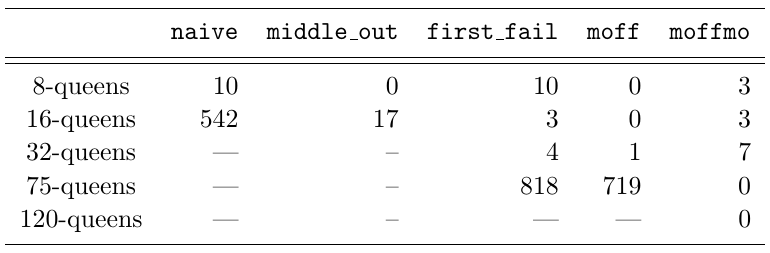
\includegraphics[scale=0.5]{HeuristicsBacktrack.png}
\end{figure}

\subsection{Outras Considerações}

O problema das n-rainhas é simétrico em que se uma solução tem a enésima rainha no emésimo quadrado da
coluna i, outra solução teria a enésima rainha na emésimo quadrado da linha i. Perceba que uma solução é
equivalente à outra, a menos de rotaçõe s de 90º. Assim, quando a heurística de ordenação de
variáveis \technical{middle\_out} sucede sem \technical{backtrackings}, a heurística de ordenação de
valores \codigo{indomain(Var, middle)} também deveria. Percebendo isso, podemos criar uma heurística
de ordenação de valores que faz \technical{backtrackings} como a \technical{middle\_out}. Depois de
aplicada, uma ``rotação'' deve nos mostrar as mesmas soluções e na mesma ordem.

Para tanto, fazemos pequenas modificações no nosso programa. No lugar de iterar sobre a lista de
variáveis, iteraremos sobre os valores do domínio. Ademais, no lugar de selecionar um valor para a
variável atual (pelo \funtor{indomain/1}), selecionaremos uma variável para um valor (pelo
\funtor{member/2}). Por fim, ``rodamos'' o resultado, para que os resultados produzidos sejam os
mesmos produzidos pelo \technical{middle\_out}. Um código representando o que foi discutido é como
segue:

    \begin{listing}
\inputminted{prolog}{../Exemplos/Cap11/prog7_queensHeurRotate.ecl}
    \caption{Heurística Roda}
    \end{listing}

Curiosamente, os resultados para o \technical{rotate} são muito melhores do que para
\technical{middle\_out}, como pode ser visto na seguinte tabela, mostrando a quantidade de
\technical{backtrackings} por N e por heurística:

\begin{figure}[h]
  \caption{Retirado de \cite{krzysztof}}\label{fig:psi}
  \centering
  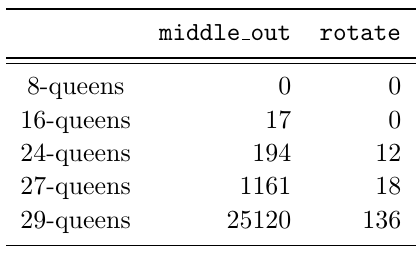
\includegraphics[scale=0.5]{rotate.png}
\end{figure}

Isso ocorre porque o comportamento da propagação de restrições não é o mesmo para linhas e colunas.
Se os valores para uma coluna são excluídos, exceto um, essa variável é instanciada ao velor
restante. Esse é o comportamento exibido por \technical{rotate}.

No entanto, no comportamento exibido por \technical{middle\_out}, se todos os valores de uma linha
são excluídos exceto um, a propagação de restrições não instancia a variável. Isso ocorre porque as
variáveis são representadas por colunas.

Uma forma de conseguir a mesma quantidade de propagação é usar uma redundância na formulação do
problema. Neste caso, poderíamos adicionar outro tabuleiro ligado ao primeiro de modo que, se uma
rainha i é posta no quadrado j de um tabuleiro, no outro, uma rainha j é posta no quadrado i.

\subsection{O Predicado Search}

Espero que a leitora não fique triste ao saber que grande parte do trabalho desenvolvido até agora
poderia ser substituído pelo uso do predicado \funtor{search/6}. Ele tem 6 argumentos:
\technical{search(+Lista, ++Arg, ++Select, +Escolha, ++Metodo, +Opcao)}. O primeiro argumento,
\var{Lista}, é uma lista de variáveis de decisão (as variáveis do problema) quando \var{Arg} é 0, ou
uma lista de funtores compostos quando $\var{Arg} > 0$. Assumiremos que \var{Arg} é 0. O argumento \var{Select}
representa uma heurística (feita pelo usuário ou não) de ordenação de variáveis, enquanto que, o
\var{Escolha}, uma de ordenação de valores. Pelo \var{Metodo}, podemos selecionar a ``forma'' pela
qual a busca deve ser feita: algumas opções são \technical{complete} (que realiza uma busca por
todos os valores), e \technical{sbds} (que faz uso da biblioteca SBDS de quebra de simetria para
excluir partes simétricas da árvore de busca)\footnote{Recomendamos a consulta ao manual do \eclipse
para mais detalhes sobre esses e outros métodos de busca}. O argumento \var{Opcao} é usado para
passar parâmetros adicionais\footnote{Novamente, é recomendado checar o manual do \eclipse para mais
informações}, algumas das quais são \technical{node(daVinci)}, para criar um desenho da
árvore de busca usando a ferramenta de desenho daVinci, e \technical{backtracks(-N)}, que nos dá em
\var{N} a quantidade de \technical{backtrackings} que ocorreram durante a busca.




  \begin{thebibliography}{2}

    \bibitem{krzysztof}
    Krzysztof R. Apt and Mark Wallace
    ``Constraint Logic Programming using ECLiPSe''
    Cambridge University Press,
    The Edinburgh Building, Cambridge CB2 8RU, UK


  \end{thebibliography}

\end{document}
